\documentclass[pdftex,12pt,a4paper]{article}

\usepackage[pdftex]{graphicx}

\newcommand{\HRule}{\rule{\linewidth}{0.5mm}}
\usepackage[danish]{babel}
\renewcommand{\danishhyphenmins}{22}
\usepackage{lmodern}
\usepackage[T1]{fontenc}
\usepackage[utf8x]{inputenc}
\usepackage[danish=quotes]{csquotes}
\usepackage{graphicx}
\usepackage{amsmath}
\usepackage{fixltx2e}
\usepackage{subfiles}
\usepackage{color}
\usepackage{tikz}
\usepackage{pdfpages}


\begin{document}

\title{Assignment 36}
\author{Tróndur Høgnason \and  Kristian Mohr Nielsen}
\date{\today}
\maketitle
\pagebreak

\section{Use-case diagram}
Our use-case diagram (figur 1) has an extra exceptional use-case, which we chose to include to make it more organized. There is two actors: the Traveler who invokes the three use-cases: BuyOneWayTicket, BuyWeeklyCard and BuyMonthlyCard, and the CentralComputerSystem who invokes the use-case UpdateTariff. Each one of the three use-cases invoked by the traveler extend DistributorException which generalises the other exceptional use-cases. This means that the three use-cases can invoke all of the exceptional use-cases
\begin{figure}[h]
\centering
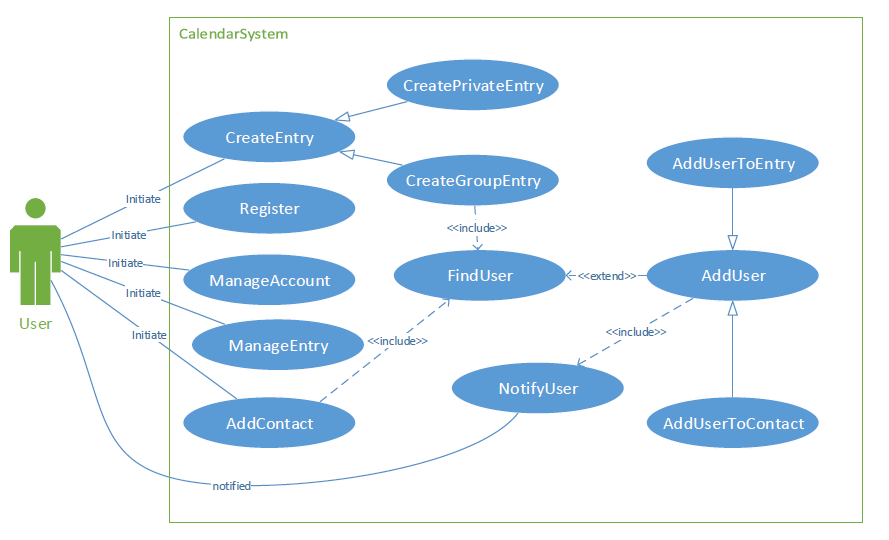
\includegraphics[scale = 0.9]{usecase.png}
\caption{Use-case diagram}
\end{figure}
\pagebreak

\section{Use cases}
Below the nine use cases are listed. Quality requirements are left blank, since there were no requirements stated in the exercise and we didn't want make something up for all of the use-cases. But some examples could be that the payment transaction needs to be completed in under xx seconds after the pin has been written. 

\subsection{Buy one way ticket}

\begin{tikzpicture}
\draw (0,0) -- (12,0);
\end{tikzpicture}

\flushleft{\textbf{Participating actors: }} \\
Communicates with Traveler
\\
\begin{tikzpicture}
\draw (0,0) -- (12,0);
\end{tikzpicture}

\flushleft{\textbf{Flow of events: }} \\
Communicates with Traveler
\\
\begin{itemize}

\item The Traveler chooses to buy one way ticket
\item The Traveler pays
\item The ticket is printed

\end{itemize}
\begin{tikzpicture}
\draw (0,0) -- (12,0);
\end{tikzpicture}

\flushleft{\textbf{Entry conditions: }} \\
The ticket distributor has change and paper
\\
\begin{tikzpicture}
\draw (0,0) -- (12,0);
\end{tikzpicture}

\flushleft{\textbf{Exit conditions: }} \\
The Traveler has received the ticket, \textbf{OR} the Traveler has received an explanation indicating why the transaction can't be completed.
\\
\begin{tikzpicture}
\draw (0,0) -- (12,0);
\end{tikzpicture}

\flushleft{\textbf{Quality requirements: }} \\
--
\\
\begin{tikzpicture}
\draw (0,0) -- (12,0);
\end{tikzpicture}
\pagebreak
\subsection{Buy weekly card}

\begin{tikzpicture}
\draw (0,0) -- (12,0);
\end{tikzpicture}

\flushleft{\textbf{Participating actors: }} \\
Initiated by Traveler
\\
\begin{tikzpicture}
\draw (0,0) -- (12,0);
\end{tikzpicture}

\flushleft{\textbf{Flow of events: }} \\
\begin{itemize}

\item The Traveler chooses to buy weekly card
\item The Traveler pays
\item The card is printed

\end{itemize}
\begin{tikzpicture}
\draw (0,0) -- (12,0);
\end{tikzpicture}

\flushleft{\textbf{Entry conditions: }} \\
The ticket distributor has change and paper
\\
\begin{tikzpicture}
\draw (0,0) -- (12,0);
\end{tikzpicture}

\flushleft{\textbf{Exit conditions: }} \\
The Traveler has received the card, \textbf{OR} the Traveler has received an explanation indicating why the transaction can't be completed.
\\
\begin{tikzpicture}
\draw (0,0) -- (12,0);
\end{tikzpicture}

\flushleft{\textbf{Quality requirements: }} \\
--
\\
\begin{tikzpicture}
\draw (0,0) -- (12,0);
\end{tikzpicture}
\pagebreak
\subsection{Buy monthly card}

\begin{tikzpicture}
\draw (0,0) -- (12,0);
\end{tikzpicture}

\flushleft{\textbf{Participating actors: }} \\
Initiated by Traveler
\\
\begin{tikzpicture}
\draw (0,0) -- (12,0);
\end{tikzpicture}

\flushleft{\textbf{Flow of events: }} \\
\begin{itemize}

\item The Traveler chooses to buy monthly card
\item The Traveler pays
\item The card is printed

\end{itemize}
\begin{tikzpicture}
\draw (0,0) -- (12,0);
\end{tikzpicture}

\flushleft{\textbf{Entry conditions: }} \\
The ticket distributor has change and paper
\\
\begin{tikzpicture}
\draw (0,0) -- (12,0);
\end{tikzpicture}

\flushleft{\textbf{Exit conditions: }} \\
The Traveler has received the card, \textbf{OR} the Traveler has received an explanation indicating why the transaction can't be completed.
\\
\begin{tikzpicture}
\draw (0,0) -- (12,0);
\end{tikzpicture}

\flushleft{\textbf{Quality requirements: }} \\
--
\\
\begin{tikzpicture}
\draw (0,0) -- (12,0);
\end{tikzpicture}
\pagebreak
\subsection{Update tariff}

\begin{tikzpicture}
\draw (0,0) -- (12,0);
\end{tikzpicture}

\flushleft{\textbf{Participating actors: }} \\
Communicates with CentralComputer
\\
\begin{tikzpicture}
\draw (0,0) -- (12,0);
\end{tikzpicture}

\flushleft{\textbf{Flow of events: }} \\
Communicates with Traveler
\\
\begin{itemize}

\item The CentralComputer updates the tariff on the distributor.

\end{itemize}
\begin{tikzpicture}
\draw (0,0) -- (12,0);
\end{tikzpicture}

\flushleft{\textbf{Entry conditions: }} \\
There has been changes to the tariff
\\
\begin{tikzpicture}
\draw (0,0) -- (12,0);
\end{tikzpicture}

\flushleft{\textbf{Exit conditions: }} \\
The Distributors tariff has been updated
\\
\begin{tikzpicture}
\draw (0,0) -- (12,0);
\end{tikzpicture}

\flushleft{\textbf{Quality requirements: }} \\
--
\\
\begin{tikzpicture}
\draw (0,0) -- (12,0);
\end{tikzpicture}
\pagebreak
\subsection{Distributor Exception}

\begin{tikzpicture}
\draw (0,0) -- (12,0);
\end{tikzpicture}

\flushleft{\textbf{Participating actors: }} \\
Communicates with Traveler
\\
\begin{tikzpicture}
\draw (0,0) -- (12,0);
\end{tikzpicture}

\flushleft{\textbf{Flow of events: }} \\
\begin{itemize}

\item This use case extends BuyOneWayTicket, BuyWeeklyCard and BuyMonthlyCard use cases. It is initiated whenever a problem occurs, as the Traveler is trying to buy a ticket.

\end{itemize}
\begin{tikzpicture}
\draw (0,0) -- (12,0);
\end{tikzpicture}
\pagebreak
\subsection{Timeout}

\begin{tikzpicture}
\draw (0,0) -- (12,0);
\end{tikzpicture}

\flushleft{\textbf{Participating actors: }} \\
Inherited from DistributorException use case
\\
\begin{tikzpicture}
\draw (0,0) -- (12,0);
\end{tikzpicture}

\flushleft{\textbf{Flow of events: }} \\
\begin{itemize}

\item Cancel transaction
\item Notify Traveler that too much time has been spent at one stage of the transaction

\end{itemize}
\begin{tikzpicture}
\draw (0,0) -- (12,0);
\end{tikzpicture}

\flushleft{\textbf{Entry conditions: }} \\
Inherited from DistributorException, \textbf{AND} XX time has been spent on one stage of the transaction.
\\
\begin{tikzpicture}
\draw (0,0) -- (12,0);
\end{tikzpicture}

\flushleft{\textbf{Exit conditions: }} \\
User has be notified
\\
\begin{tikzpicture}
\draw (0,0) -- (12,0);
\end{tikzpicture}
\pagebreak
\subsection{Transaction aborted}

\begin{tikzpicture}
\draw (0,0) -- (12,0);
\end{tikzpicture}

\flushleft{\textbf{Participating actors: }} \\
Inherited from DistributorException use case
\\
\begin{tikzpicture}
\draw (0,0) -- (12,0);
\end{tikzpicture}

\flushleft{\textbf{Flow of events: }} \\
\begin{itemize}

\item Cancel transaction
\item Notify the traveler that the transaction has been aborted

\end{itemize}
\begin{tikzpicture}
\draw (0,0) -- (12,0);
\end{tikzpicture}

\flushleft{\textbf{Entry conditions: }} \\
Some event has aborted the transaction
\\
\begin{tikzpicture}
\draw (0,0) -- (12,0);
\end{tikzpicture}

\flushleft{\textbf{Exit conditions: }} \\
Traveler has been notified
\\
\begin{tikzpicture}
\draw (0,0) -- (12,0);
\end{tikzpicture}

\flushleft{\textbf{Quality requirements: }} \\
--
\\
\begin{tikzpicture}
\draw (0,0) -- (12,0);
\end{tikzpicture}
\pagebreak
\subsection{Distributor out of paper}

\begin{tikzpicture}
\draw (0,0) -- (12,0);
\end{tikzpicture}

\flushleft{\textbf{Participating actors: }} \\
Inherited from DistributorException use case
\\
\begin{tikzpicture}
\draw (0,0) -- (12,0);
\end{tikzpicture}

\flushleft{\textbf{Flow of events: }} \\
\begin{itemize}

\item Notify the traveler that the distributor is out of paper

\end{itemize}
\begin{tikzpicture}
\draw (0,0) -- (12,0);
\end{tikzpicture}

\flushleft{\textbf{Entry conditions: }} \\
The distributor is out of paper
\\
\begin{tikzpicture}
\draw (0,0) -- (12,0);
\end{tikzpicture}

\flushleft{\textbf{Exit conditions: }} \\
The distributor has been refilled with paper
\\
\begin{tikzpicture}
\draw (0,0) -- (12,0);
\end{tikzpicture}

\flushleft{\textbf{Quality requirements: }} \\
--
\\
\begin{tikzpicture}
\draw (0,0) -- (12,0);
\end{tikzpicture}
\pagebreak
\subsection{Distributor out of change}

\begin{tikzpicture}
\draw (0,0) -- (12,0);
\end{tikzpicture}

\flushleft{\textbf{Participating actors: }} \\
Inherited from DistributorException use case
\\
\begin{tikzpicture}
\draw (0,0) -- (12,0);
\end{tikzpicture}

\flushleft{\textbf{Flow of events: }} \\
\begin{itemize}

\item Notify the traveler that the distributor is out of change

\end{itemize}
\begin{tikzpicture}
\draw (0,0) -- (12,0);
\end{tikzpicture}

\flushleft{\textbf{Entry conditions: }} \\
The distributor is out of change
\\
\begin{tikzpicture}
\draw (0,0) -- (12,0);
\end{tikzpicture}

\flushleft{\textbf{Exit conditions: }} \\
The distributor has been refilled with change
\\
\begin{tikzpicture}
\draw (0,0) -- (12,0);
\end{tikzpicture}

\flushleft{\textbf{Quality requirements: }} \\
--
\\
\begin{tikzpicture}
\draw (0,0) -- (12,0);
\end{tikzpicture}
\pagebreak

\section{Class diagram}
Our class diagram (figur 2) is of the distributor and its parts, although simple. We've chosen that it has: a touch display, for input and output of information, two terminals - one for paying with card and another for paying with cash and finally it has a printer to print the pass (a ticket or a card).
\begin{figure}[h]
\centering
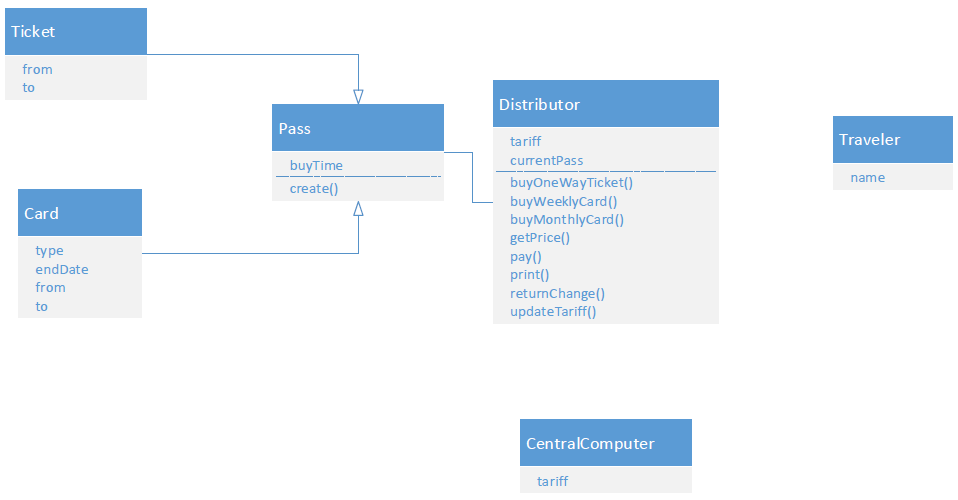
\includegraphics[scale = 0.9]{class.png}
\caption{Class diagram}
\end{figure}

\pagebreak

\section{Sequence diagram}
We've chosen to make a sequence diagram for the  interaction between a traveler, the distributor and parts of the distributor (figur 3), when the traveler buys a pass (a ticket or a card).
\begin{figure}[h]
\centering
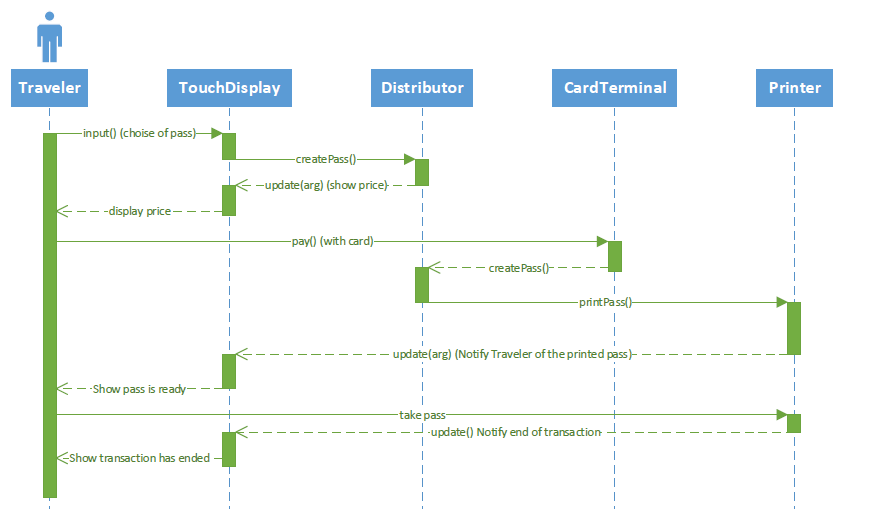
\includegraphics[scale = 0.7]{sequence.png}
\caption{Sequence diagram}
\end{figure}

\pagebreak

\section{Activity diagram}
Figure 4 shows our activity diagram of a traveler buying a pass. First the traveler has to choose which kind of pass he wants to buy, then the traveler can choose to pay with either card or cash. After paying the ticket is printed and the traveler can take it. If there is any change the traveler picks it up (at least in a perfect world) and the transaction is over.
\begin{figure}[h]
\centering
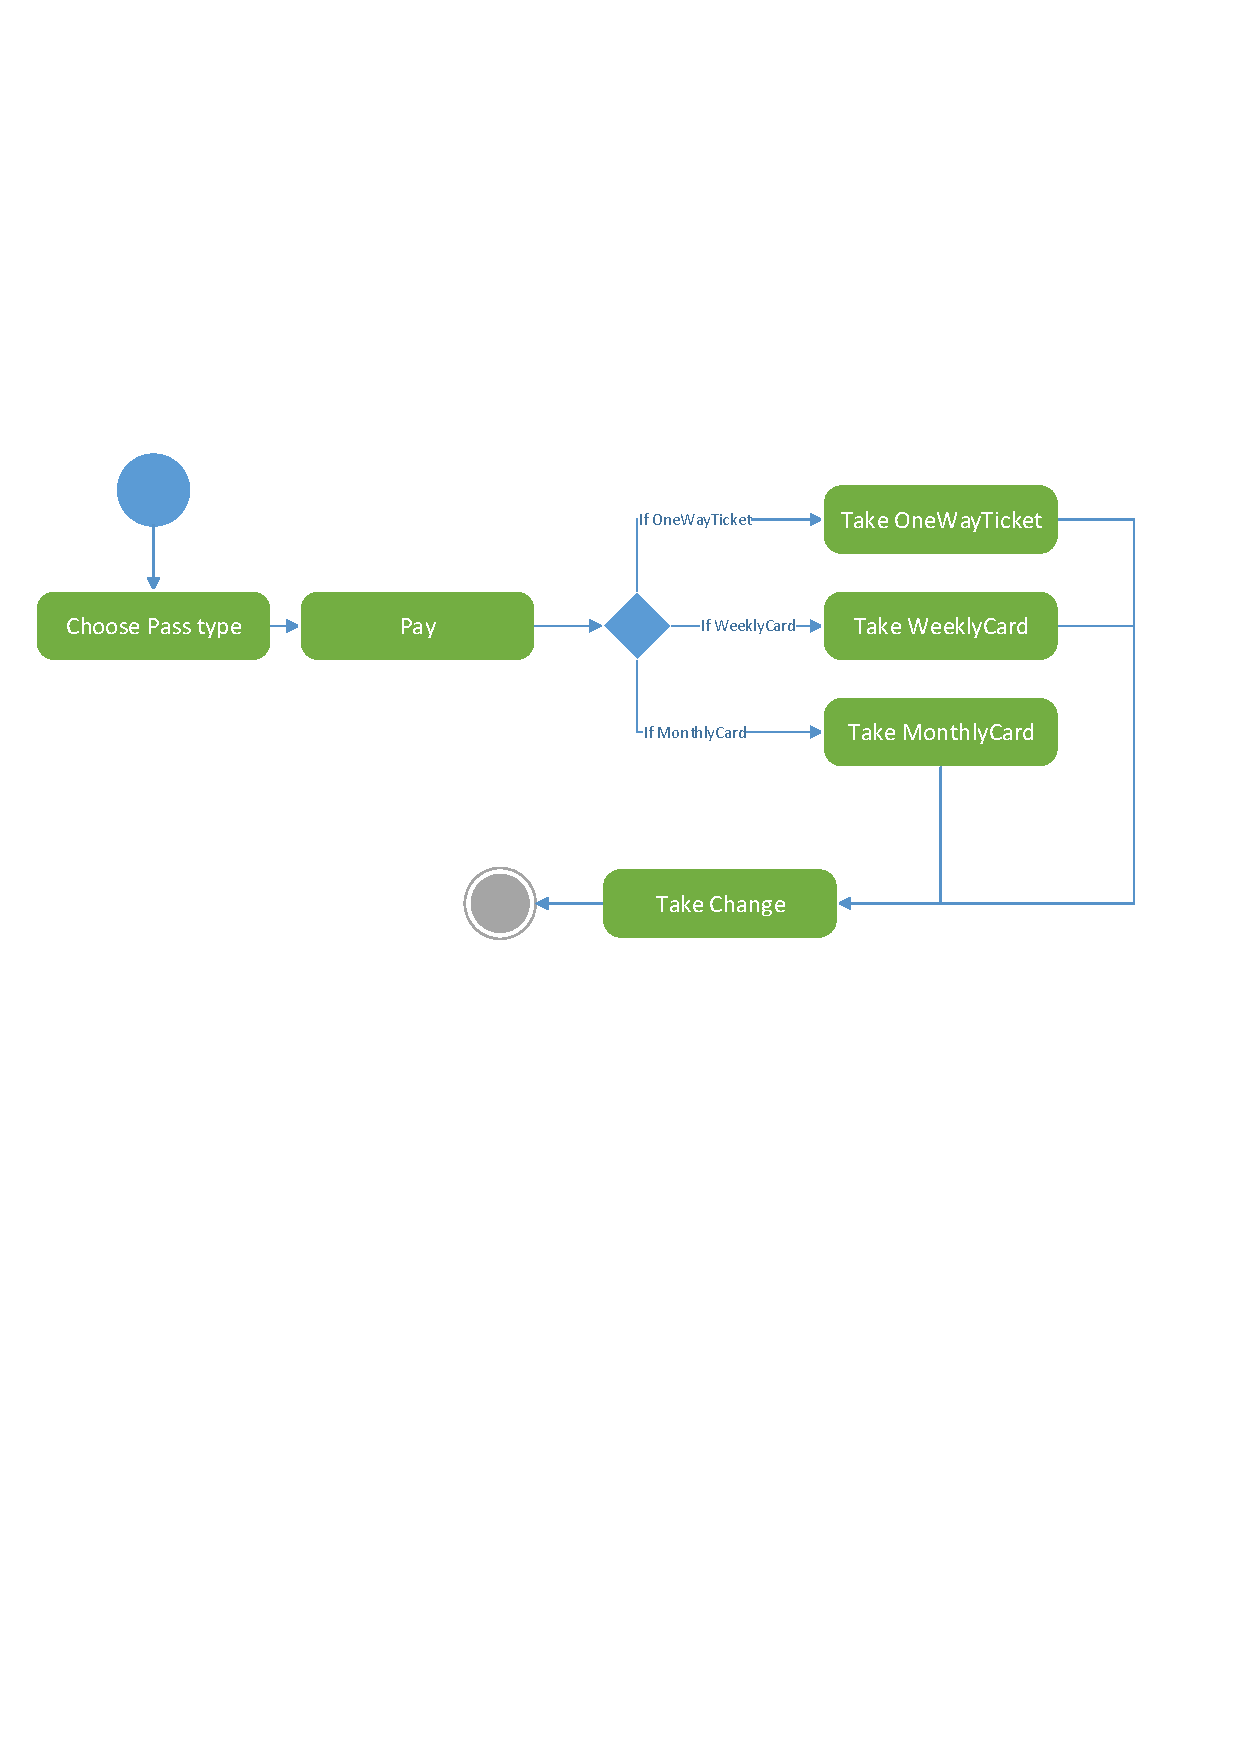
\includegraphics[scale = 0.8]{activity.png}
\caption{Activity diagram}
\end{figure}

\end{document}